\documentclass[11pt,a4paper]{scrartcl} 

% Kalbos nustatymai (lietuvių kalbai)
\usepackage[utf8]{inputenc}
\usepackage[T1]{fontenc}
\usepackage{tasks}
\usepackage{tikz}
\usepackage{lmodern} % Įkeliame modernų šriftą, kuris palaiko visas reikalingas formas
\usepackage[lithuanian]{babel}

% Įkeliame jūsų .sty failą (įsitikinkite, kad Overleaf projekte šalia yra failas manostilius.sty)
\usepackage{../manostilius_lt}

% Projekto informacija (būtina preambulėje dėl jūsų stiliaus specifikos)
\title{Algebriniai reiškiniai}
\author{Andrius Berniukevičiuss} 

\begin{document}

\maketitle


\section{Algebrinių reiškinių tipai}
\vocab{Algebriniai reiškiniai} yra pagrindiniai matematikos kalbos elementai, kuriuose skaičiai ir 
kintamieji jungiami aritmetiniais veiksmais. Norint sėkmingai atlikti veiksmus su algebriniais reiškiniais, 
būtina suprasti jų struktūrą ir savybes. Šiame skyriuje susipažinsime 
su algebrinių reiškinių klasifikacija, išmoksime juos atpažinti ir skirstyti į atitinkamas kategorijas.


\begin{definition}
    \vocab{Algebrinis reiškinys} – tai matematinis užrašas, sudarytas iš skaičių ir kintamųjų (raidžių), sujungtų aritmetinių veiksmų (sudėties, atimties, daugybos, dalybos, kėlimo laipsniu ar šaknies traukimo) ženklais. Reiškiniuose taip pat gali būti naudojami skliaustai, nurodantys veiksmų atlikimo tvarką.
\end{definition}

\begin{example}
Štai atskiri algebrinių reiškinių pavyzdžiai, iliustruojantys kiekvieną pagrindinį matematinį veiksmą:
\begin{itemize}
    \item \textbf{Sudėtis ir atimtis:} 
    \[ 3x + 5y - 7 \]
    
    \item \textbf{Daugyba:} 
    \[ 4a(a - 2b) \]
    
    \item \textbf{Dalyba (trupmena):} 
    \[ \frac{2x - 1}{x + 4} \]
    
    \item \textbf{Kėlimas laipsniu:} 
    \[ 5x^4 - 2x^2 + 8 \]
    
    \item \textbf{Šaknies traukimas:} 
    \[ \sqrt{x^2 + y^2} \]
\end{itemize}
\end{example}

Algebriniai reiškiniai skirstomi į \textbf{racionalius} ir \textbf{irracionalius} reiškinius pagal tai, ar su bent vienu kintamuoju yra atliekamas šaknies traukimo veiksmas.
\begin{definition}
    \vocab{Racionalus reiškinys} - tai algebrinis reiškinys, kuriame su kintamaisiais (raidėmis) atliekami tik šie veiksmai: sudėtis, atimtis, daugyba, dalyba ir kėlimas sveikuoju laipsniu. Juose nėra šaknies traukimo iš kintamojo veiksmo.
\end{definition}
\begin{example}
Racionaliųjų reiškinių pavyzdžiai:
    \begin{itemize}
        \item $3x ^{2} -5$
        \item $\frac{a+b}{c} $
        \item $(x-2)(x+3)$ 
    \end{itemize}
\end{example}

\begin{definition}
    \vocab{Irracionalus reiškinys} - tai algebrinis reiškinys, kuriame bent vienas kintamasis (raidė) yra po šaknies ženklu arba yra keliamas trupmeniniu laipsniu.
\end{definition}
\begin{example}
Racionaliųjų reiškinių pavyzdžiai:
    \begin{itemize}
        \item $5\sqrt{a}+5b $
        \item $ \frac{4}{\sqrt[3]{x+y} }  $
        \item $x ^{\frac{1}{3}} +4x-5   $ 
    \end{itemize}
\end{example}
\begin{remark}
    Reiškinys $\sqrt{5}x-3y$ nėra irracionalus, nes po šaknimi yra skaičius, o ne kintamasis.
\end{remark}

\textbf{Racionalieji reiškiniai} yra skirstomi \textbf{sveikus} ir \textbf{trupmeninius} reiškinius pagal tai, ar juose yra dalyba iš kintamojo.


\begin{definition}
    \vocab{Sveikas reiškinys} - tai racionalus reiškinys, kuris neturi dalybos iš kintamojo.
\end{definition}

\begin{example}
Sveikų reiškinių pavyzdžiai:
    \begin{itemize}
        \item $7x ^{3} -4x+1$
        \item $(a+2b) ^{3} $
        \item $\frac{x+3}{7} $ 
    \end{itemize}
\end{example}

\begin{definition}
    \vocab{Trupmeninis reiškinys} - tai racionalus reiškinys, kuriame yra dalyba iš kintamojo
\end{definition}

\begin{example}
Trupmeninių reiškinių pavyzdžiai:
    \begin{itemize}
        \item $\frac{5}{x}+x-8$
        \item $\frac{a+b}{a-b}  $
        \item $\frac{5}{x-3}+ \frac{1}{x}  $ 
    \end{itemize}
\end{example}
\begin{remark}
    Nors reiškinyje $4x^{-2} $ dalybos tiesiogiai nematome, tai nėra racionalus reiškinys, nes:
    $$4x ^{-2} = 4 \cdot \frac{1}{x ^{2} }  = \frac{4}{x ^{2} }   $$
    Kadangi vardiklyje yra kintamasis, vadinasi, tai yra trupmeninis reiškinys.
\end{remark}

Visų algebrinių reiškinių klasifikacijos medis:

\begin{center}
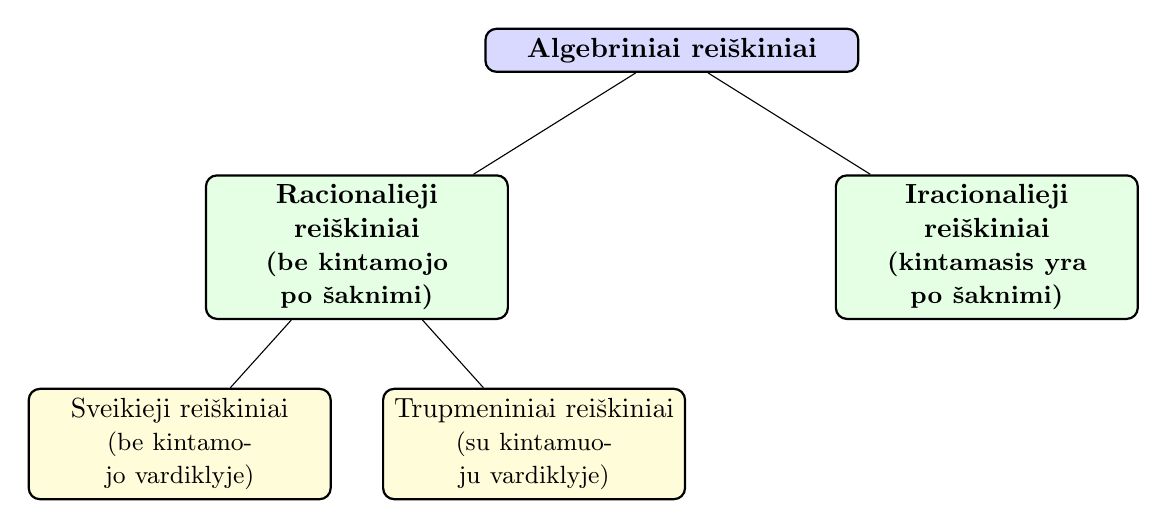
\begin{tikzpicture}[
  % Atstumai tarp lygių ir šakų
  level distance=2.5cm,          % Šiek tiek padidintas gylis, kad tekstas turėtų erdvės
  level 1/.style={sibling distance=8.0cm},
  level 2/.style={sibling distance=4.5cm},
  % Bendras mazgų stilius
  every node/.style={draw, rectangle, rounded corners, text width=3.6cm, align=center, thick},
  % Specifiniai stiliai skirtingiems lygiams (su spalvomis)
  root/.style={fill=blue!15, text width=4.5cm, font=\bfseries},
  level1/.style={fill=green!10, font=\bfseries},
    level2/.style={fill=yellow!15}
]

  % Medžio braižymas
  \node[root] {Algebriniai reiškiniai}
    child {node[level1] {Racionalieji reiškiniai \\ \small(be kintamojo po šaknimi)}
            child {node[level2] {Sveikieji reiškiniai \\ \small(be kintamojo vardiklyje)}}
      child {node[level2] {Trupmeniniai reiškiniai \\ \small(su kintamuoju vardiklyje)}}
    }
    child {node[level1] {Iracionalieji reiškiniai \\ \small(kintamasis yra po šaknimi)}};

\end{tikzpicture}
\end{center}


\section{Uždaviniai}
\begin{problem}
Prie kiekvieno žemiau esančio reiškinio parašykite, kokio tipo tai reiškinys: racionalus, iracionalus, sveikas ar trupmeninis. Atsiminkite, kad reiškinys gali turėti daugiau nei vieną tipą.

\begin{tasks}[ label={(\arabic*)},label-offset=0.9em](4) % Nustatome skaičiavimą ir formatą (1)
    \task $7x^3 -x- 15$
    \task $\sqrt{ab} + 5$
    \task $\frac{7x}{3}$
    \task $\frac{5}{y ^{3} }$
    %
    \task $-6a^3bc ^{2} $
    \task $x^2 + 2xy + y^2$
    \task $\sqrt{7}x - 2x ^{4} $
    \task $5a^{-3}$
    %
    \task $12$
    \task $\frac{x+3}{x-3}$
    \task $y^{\frac{2}{3}} + 5y$
    \task $\frac{x-1}{3} + 4x$
    %
    \task $abcd$
    \task $\frac{1}{\sqrt[3]{x}+2}$
    \task $(x-2)^3$
    \task $-\frac{3}{5}m^2n$
    %
    \task $x + 8$
    \task $(x+3)(x-2)$
    \task $\frac{4}{x^2}$
    \task $a^2 - b^2$
\end{tasks}
\end{problem}

\newpage
\section{Atsakymai}
\begin{tasks}[label={(\arabic*)}, label-offset=0.9em](1)
    \task racionalus, sveikas.
    \task iracionalus (kintamieji po šaknimi).
    \task racionalus, sveikas.
    \task racionalus, trupmeninis (kintamasis vardiklyje).
    \task racionalus, sveikas.
    \task racionalus, sveikas.
    \task racionalus, sveikas (po šaknimi tik skaičius).
    \task racionalus, trupmeninis (lygu $\frac{5}{a^3}$).
    \task racionalus, sveikas.
    \task racionalus, trupmeninis.
    \task iracionalus (trupmeninis laipsnis).
    \task racionalus, sveikas.
    \task racionalus, sveikas.
    \task iracionalus (kintamasis po šaknimi).
    \task racionalus, sveikas.
    \task racionalus, sveikas.
    \task racionalus, sveikas.
    \task racionalus, sveikas.
    \task racionalus, trupmeninis.
    \task racionalus, sveikas.
\end{tasks}




\end{document}